\section{Implementation}

In this section we will discuss our attempt in recreating the HuddleLamp project but without the use of a camera. 


\subsection{Architecture} \label{nocamer_architecture}

We plan to have an arrangement of having at least three Bluetooth Beacons around the table as shown in Figure \ref{fig:nocamera}. Using those Beacons as reference nodes we are hoping to calculate the position of a device on the table using the trilateration position algorithm.
 
 \begin{figure}
 \centering
 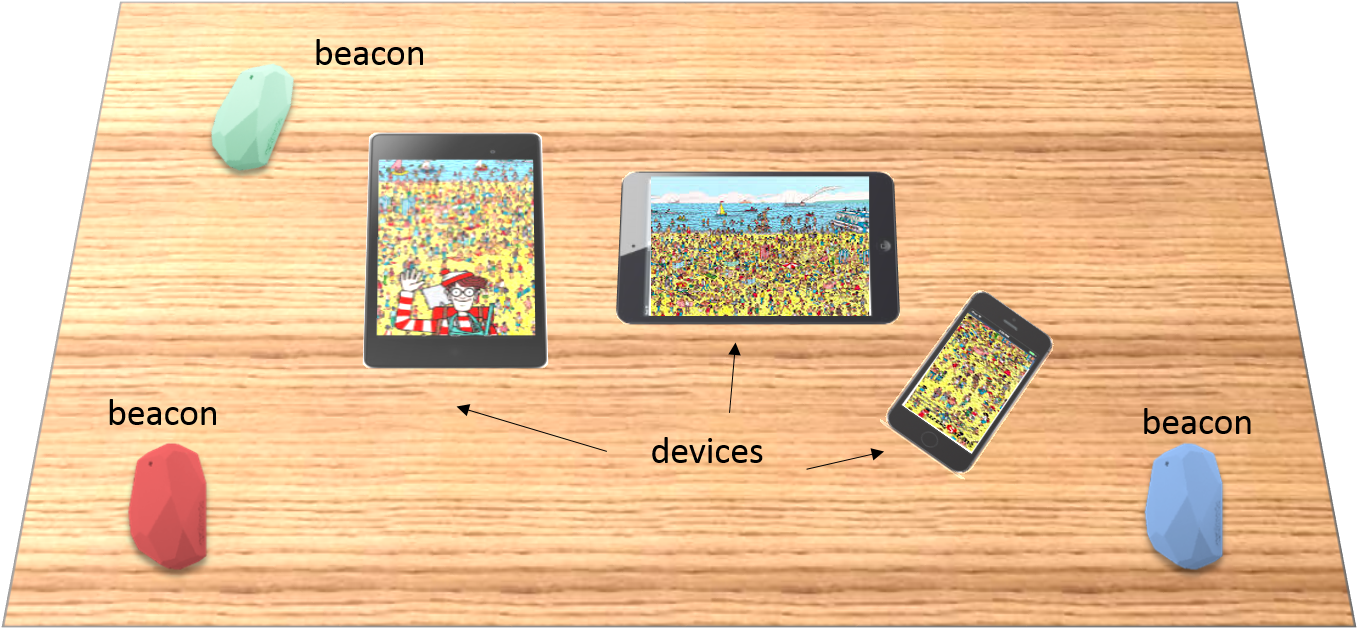
\includegraphics[scale=0.5]{nocamera}
 \caption{The arrangement of the No Camera implementation}
 \label{fig:nocamera}
 \end{figure}

\subsection{Applications}
Our research into Bluetooth Low Energy (BLE) technology has shown us that there are more than one way to work out the distance between the device emitting the BLE signal and the receiver. 
\begin{enumerate}
\item Accuracy
\item RSSI signal
\end{enumerate}
Most BLE libraries have a method which gives the distance from the beacon to device called Accuracy. Accuracy is a term coined by Apple for their CoreLocation framework to define the distance in meters from the beacon. For Estimote Beacons the method is called  \lstinline|computeAccuracy()|. Similar to the Apple function, the calculation done to get this result is hidden by Estimote in their library. However investigation into some open source libraries \cite{radius-ranging, android_ibeacon_alt} we can make an educated guess that the distance was calculated by observing RSSI and TxPower (Transmission Power) values at certain distance intervals and making a line of best fit.

The second option is for us is to redo the observation, to get the resulting RSSI signal and TxPower, for a subset of distances and get a line of best fit. We could use this information to detemine the relationship between the RSSI reading and Transmission power to calculate the distance. However this would mean that the library would be tailored to the set of beacons we have, instead of being a general library. This would be defeating the point of our project. However in section \ref{nocamera-eval} we will see how both types of distancing was required.

\subsubsection{Distance App} \label{nocamera_distanceapp}
Initially we created an application which showed the distance, between the beacon and the device, using \lstinline|computeAccuracy()| method. Figure \ref{distance_app_image} shows the UI for the application. It shows the list, ordered by the distance, of nearby beacons. It also shows other information such as the RSSI value, Transmission Power and meta data like mac address of the devices from every BLE reading.
It is a list that keeps updating all of its values on the arrival of new BLE packets.

\begin{figure}[h]
\centering
  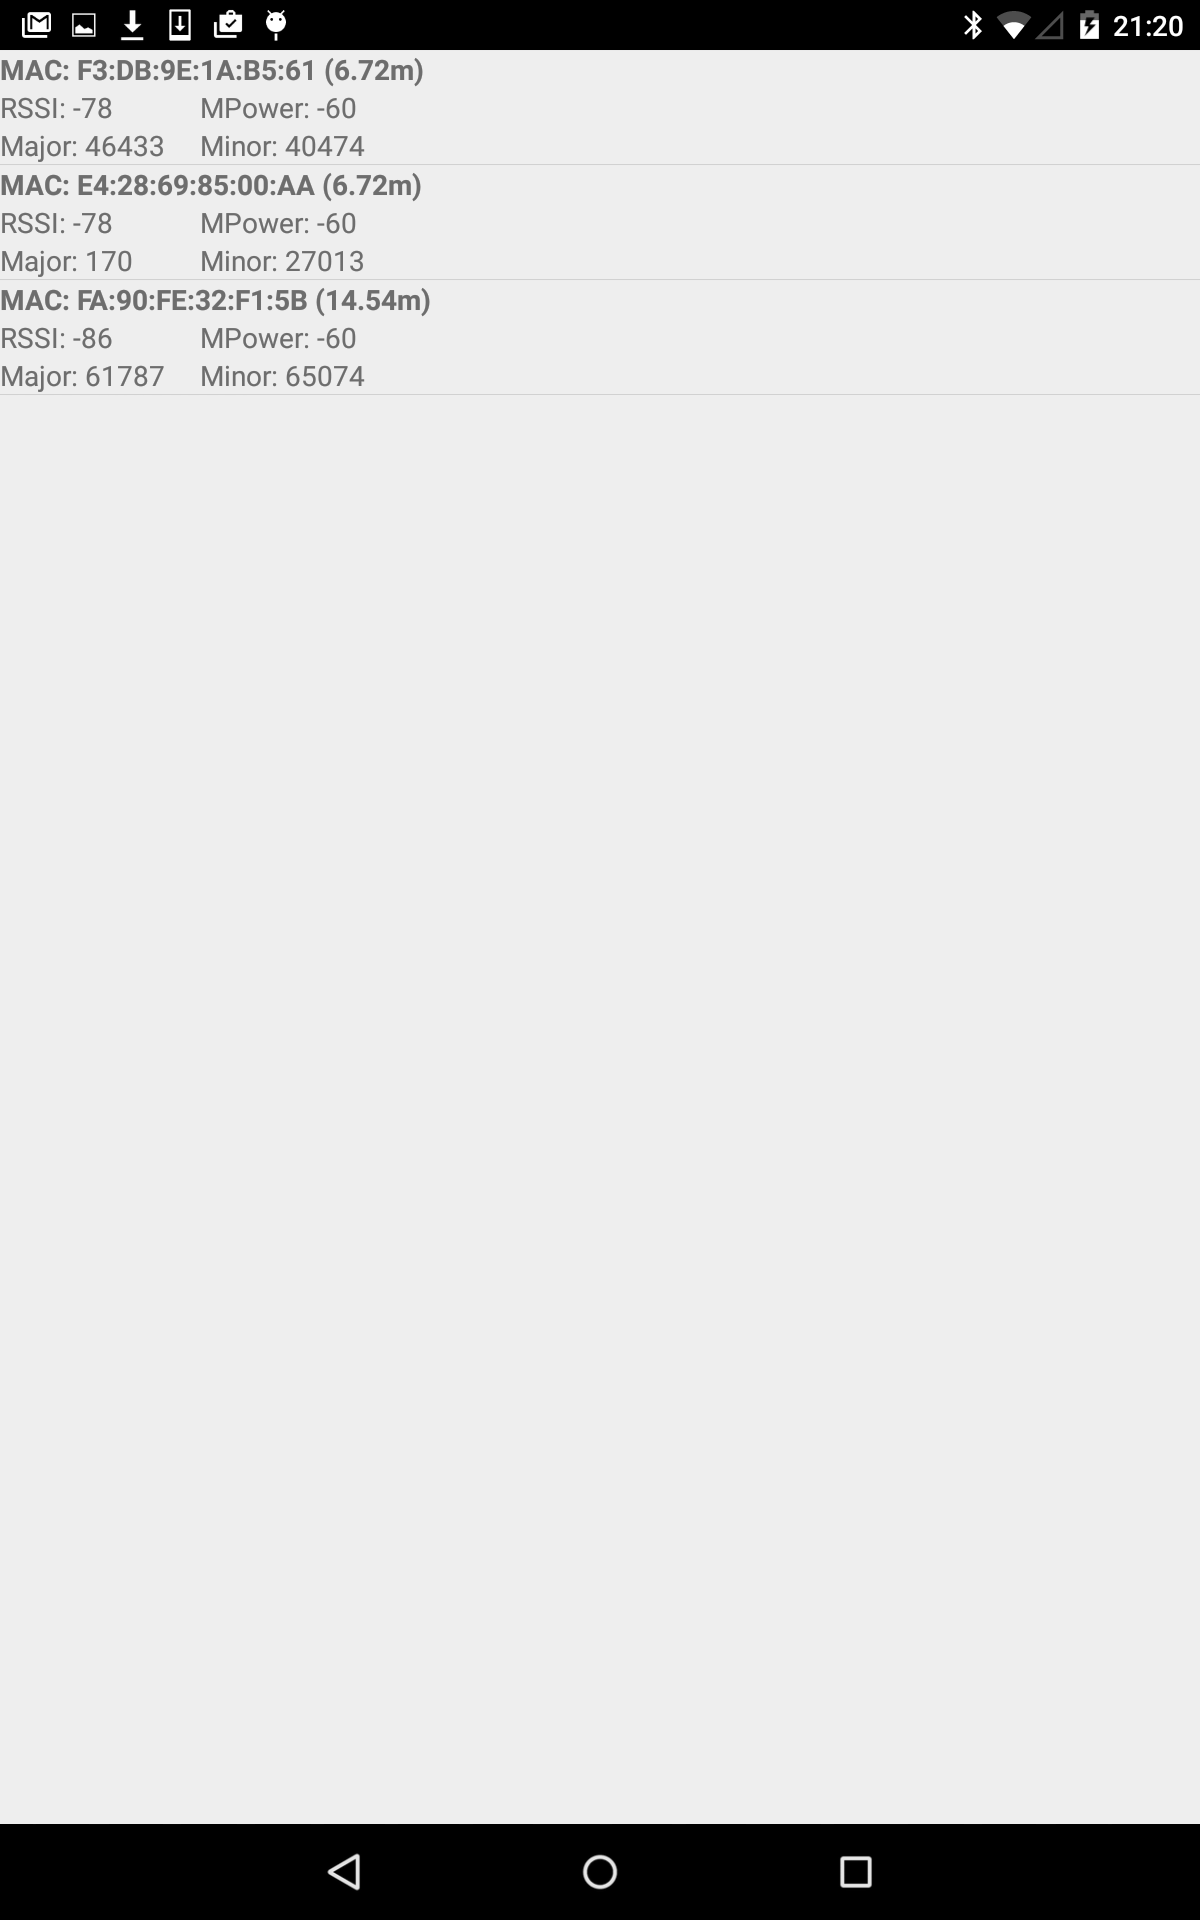
\includegraphics[scale=0.2]{images/distance}
  \protect\caption{Distance App} 
  \label{distance_app_image}
\end{figure}

\subsubsection{Trilateration} \label{nocamera_trilateration}

By creating the Distance app, we were able to familiarise ourselves with the Estimote library. This aided us in creating the trilateration part of the library. We decided to stick to a Cartesian coordinate system for our design and created a \lstinline|Position| class which kept track of the x and y position of the devices on the table. We also created a \lstinline|FixedBeacon| class which stored the reference beacon and its location.

Using these new additions we were able to create a method that calculates the position of the devices on the table. \lstinline|Position calculatePosition(List<FixedBeacon> beaconList)| It requires a list of reference beacons, of size three, and calculate the distance to those reference beacons. It uses the calculation shown in Figure \ref{psuedo-code} to determine the position of the receiver. 

Figure \ref{trilateration} shows the output of the calculation in the UI we created.
\begin{figure}[h]
\centering
  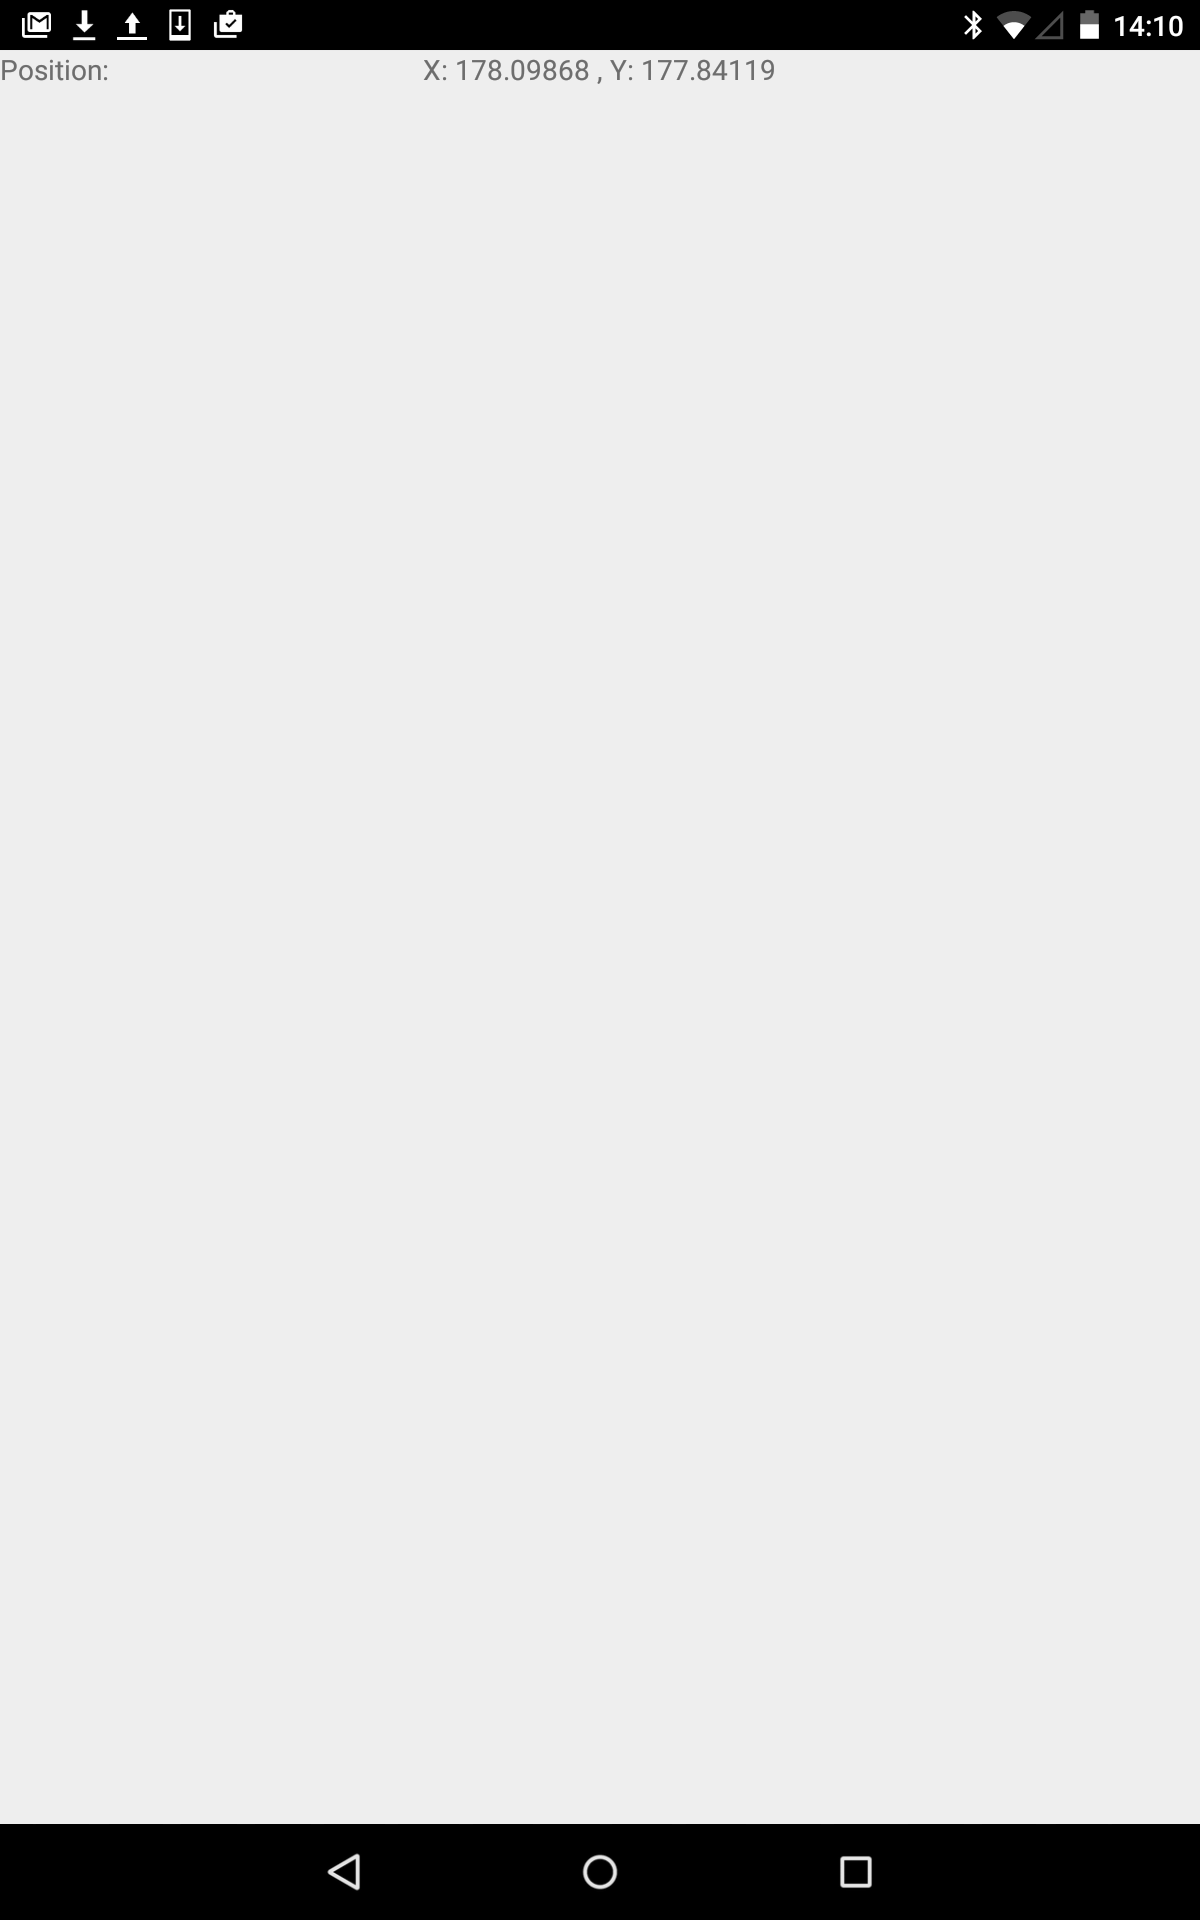
\includegraphics[scale=0.2]{images/trilateration}
  \protect\caption{Trilateration UI showing the x and y position of the device}
  \label{trilateration}
\end{figure}

\subsubsection{Sensors} \label{nocamera_sensors}
During the implementation and evaluation of the Distance app and Trilateration app, it was clear that something else needs to be combined with BLE for the positioning system to improve its accuracy. Therefore, inspired by the Hybrid sensing method used by HuddleLamp, we decided to add an accelerometer to our system. We hope that the accelerometer values, which calculates the movement, in addition to the BLE trilateration result combined should cancel out some errors, creating a more accurate positioning system. Even though most devices have a gyroscope, the use cases of our library did not require the device to be tilted in any way hence gyroscope was not necessary. 

On a stationary device there is always an acceleration of 1g (9.81 m/s \textsuperscript{2} )
in the z axis due to the effect of gravity on the device. Therefore we required a calibration step for our sensor, which would aid to eradicate any systematic error we might have. During our calibration step our application polls the sensor for one second, while keeping our device stationary, and calculate the average acceleration value in all 3 axes. This value will be taken away from any values given by the accelerometer.

As you can see from our research into sensors, in section \nameref{accelerometer}, the process of calculating displacement from accelerometer values is by integrating the values twice\ref{double_integration}. After doing some research into numerical integration methods, the most simple integration method was the ideal one to use as a proof of concept. We used a simple trapezium rule where we averaged the acceleration value for each second and then integrated it twice by getting the area under the curve for that second twice. By using fixed variables it was possible to change the chunk sizes from 1 second to something smaller if more finer results were required.
Figure \ref{sensor_app_image} shows the UI of the application that displays the accelerometer values in x, y and z axis and also the displacement in the x and y axis.

\begin{figure}[h]
\centering
    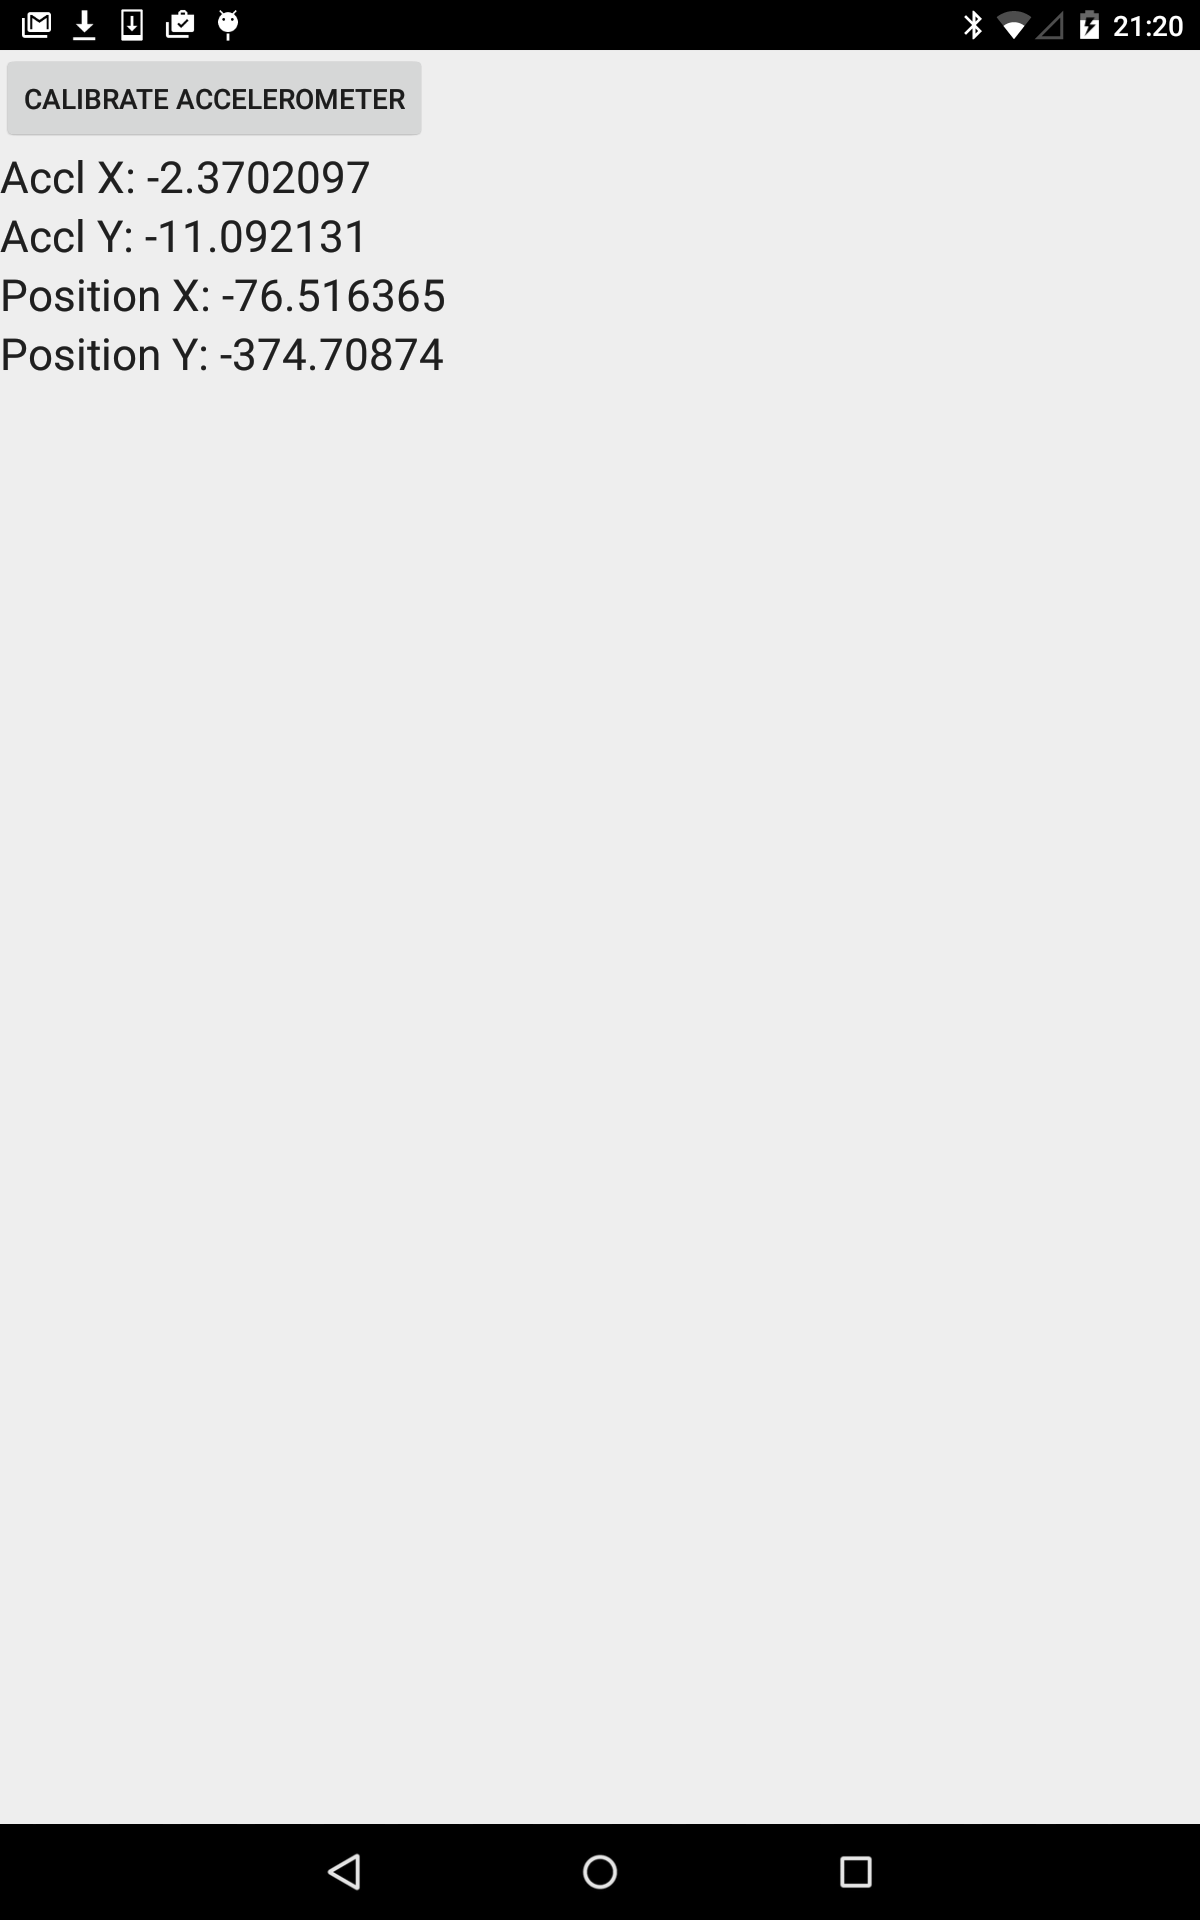
\includegraphics[scale=0.2]{images/sensor}
    \protect\caption{Sensor App} 
    \label{sensor_app_image}
\end{figure}


\subsection{Where's Wally}
One of the main features promoted by the HuddleLamp project was following the map and Where's Wally game application that they have created. As an application that shows all the advantages of the HuddleLamp project and also an impressive demonstration of the power of the project, we decided to recreate the Where's Wally game using our new positioning system. 

However during the evaluation of the functions we realised that positioning algorithm is not accurate enough. Therefore this line of investigation in an attempt to take way the camera and the laptop was futile. This would be explained in depth in Section \ref{nocamera-eval}

\begin{figure}[h]
\centering
  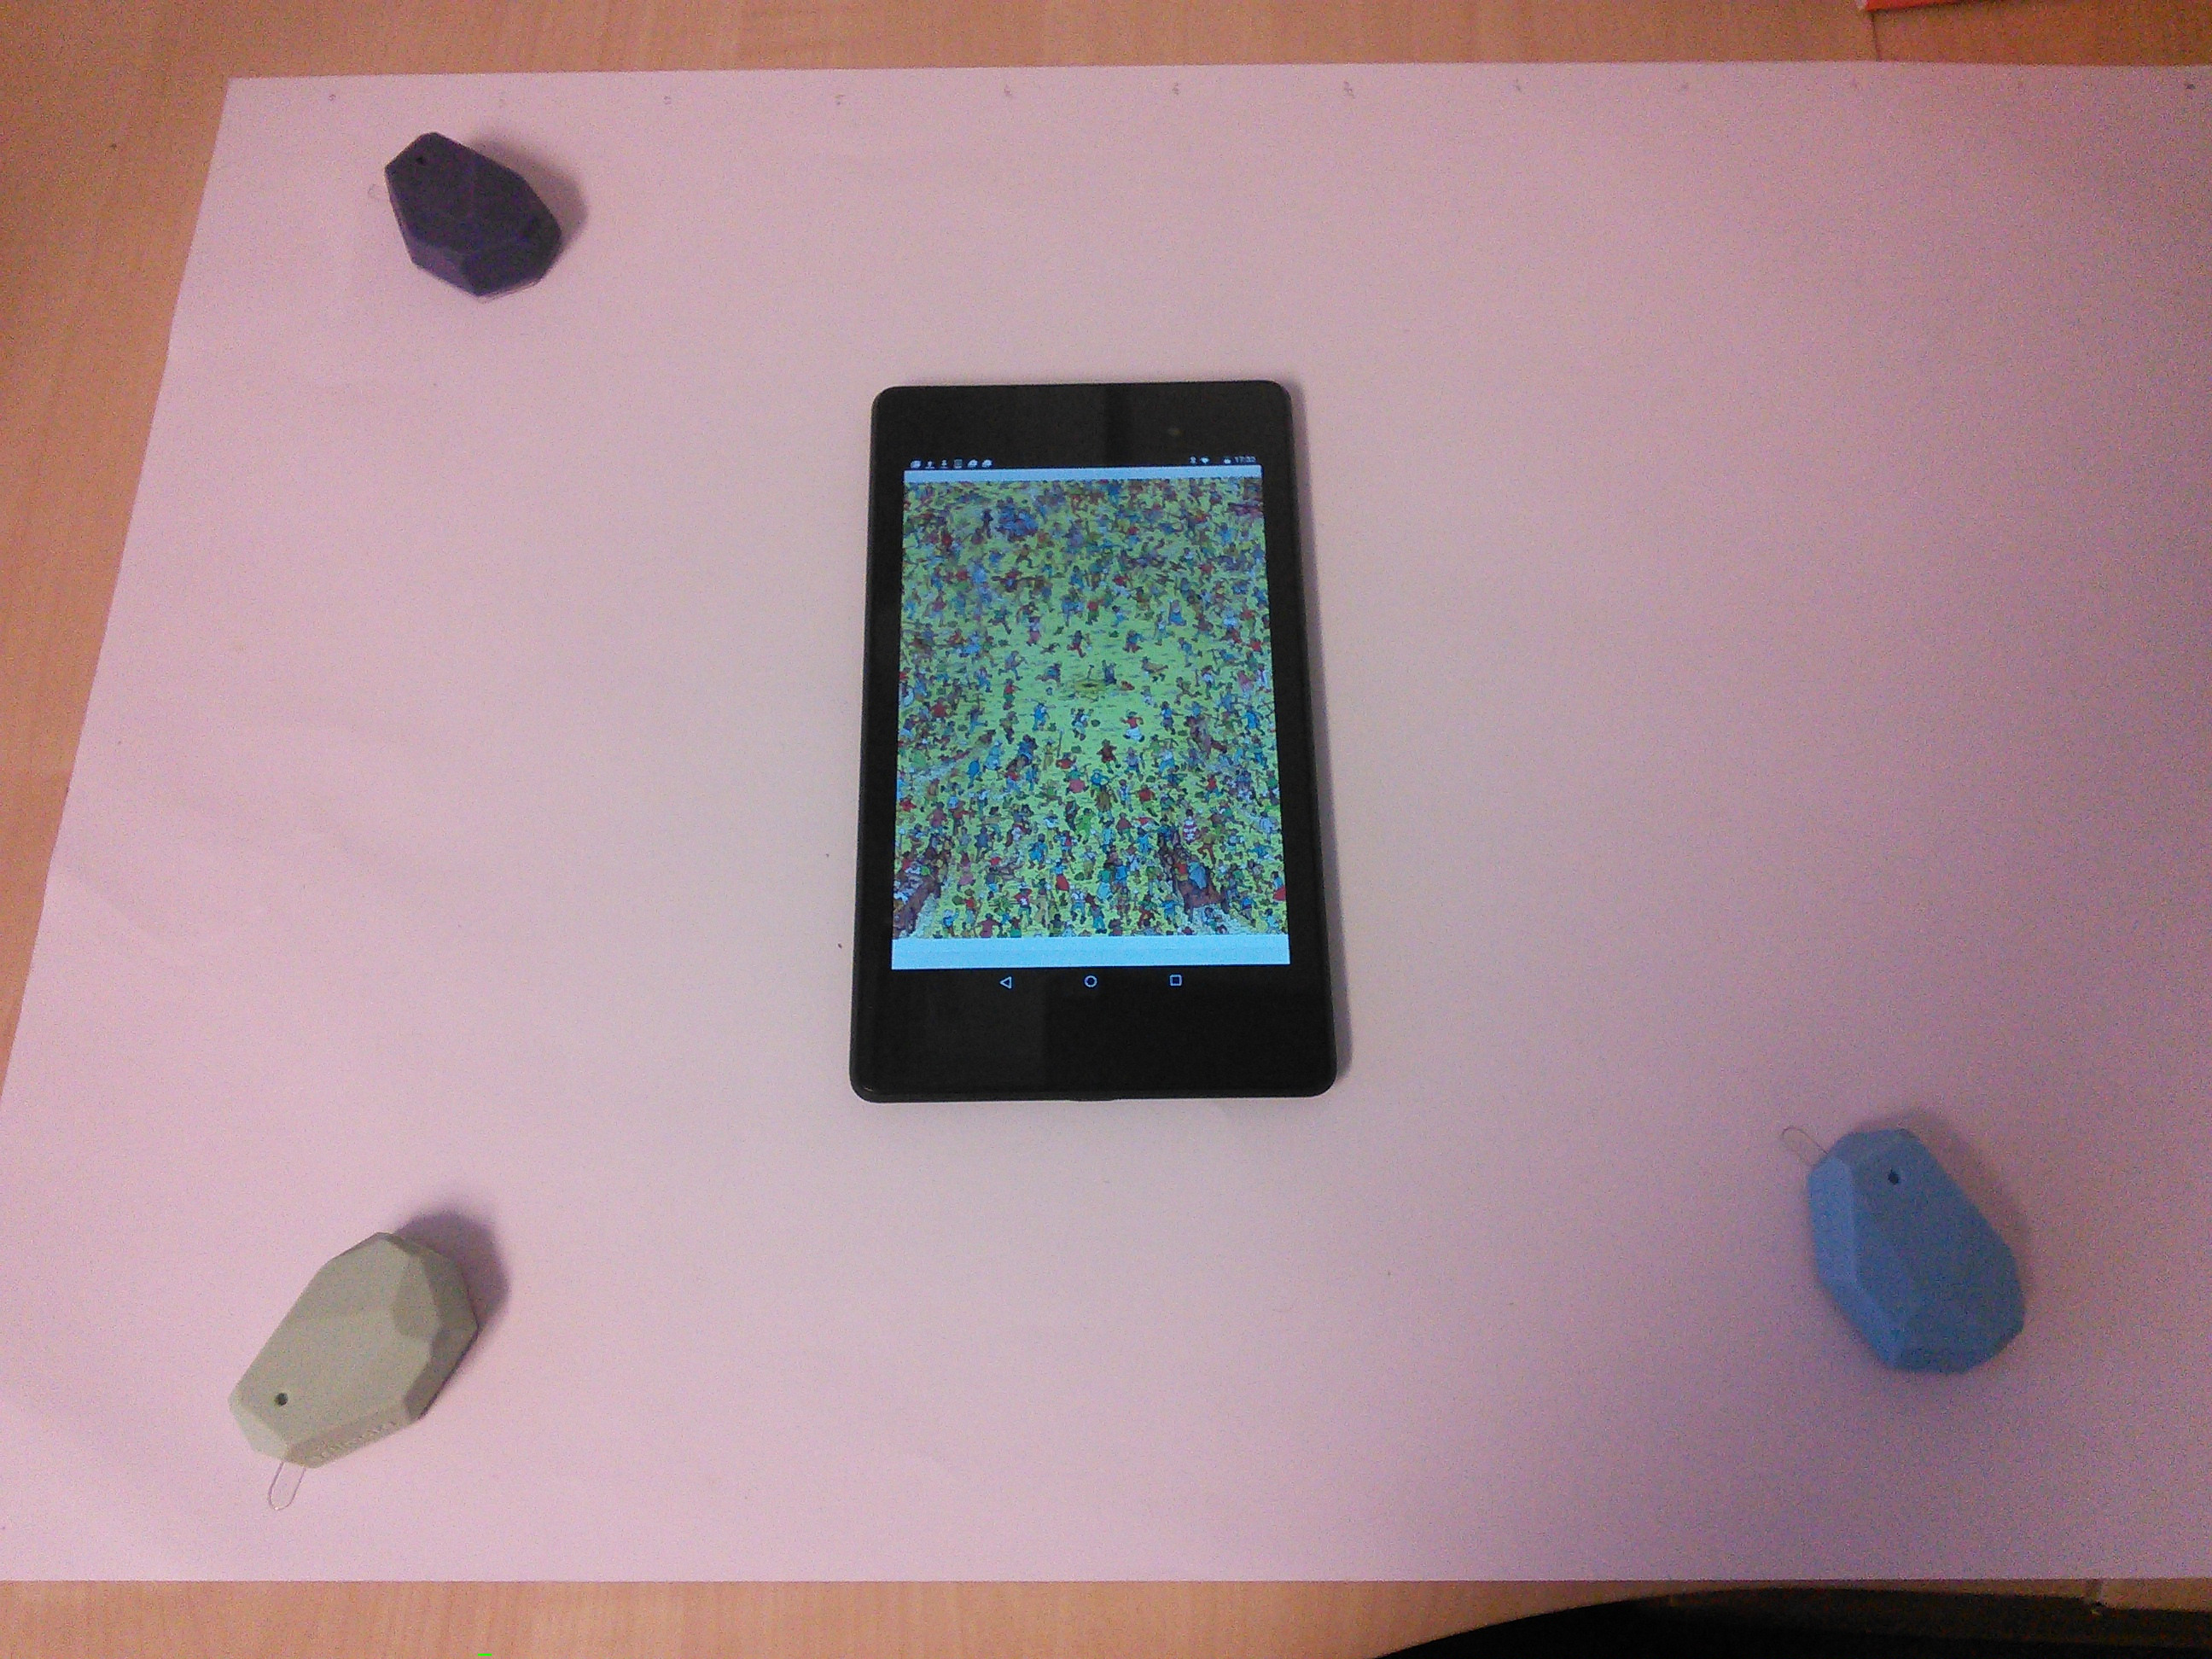
\includegraphics[scale=0.1]{images/setup}
  \protect\caption{Where is Wally App} 
  \label{where_is_wally_setup}
\end{figure}

\subsection{Canvas}
We also created a CanvasApp which harnessed the full potential of Firebase for this project. This application is similar to a paint application that a user might have. It is aimed at designers wanting to work on a particular part of large canvas. Enabling collaboration with different people, to work on the same graphic. Multiple people collaborating on the same document at the same time is one of the problems we wanted to tackle within this project. It was an aspect that was not advertised too much with HuddleLamp and has a potential to be a useful product. 
By utilising the facilities of Firebase and building on their sample project\cite{firebase-drawing}, we were able to create the Canvas Application. We were able to initialise the application with a large drawable canvas. We were then able to use the TouchSensor on the Android device to get the position of the user interactions on the screen. Combining that with the position of the device on the table using our positioning algorithm we were able to save the location of all the vector graphic lines that were drawn on the application.


